% Build:  python scripts/make_report_assets.py   (tables, figures, numbers from results/)
%         cd report && tectonic main.tex
\documentclass[11pt,letterpaper]{article}

\usepackage[margin=1in]{geometry}
\usepackage[T1]{fontenc}
\usepackage{lmodern}
\usepackage{microtype}
\usepackage{amsmath,amssymb}
\usepackage{booktabs}
\usepackage{array}
\usepackage{float}
\usepackage{graphicx}
\usepackage{xcolor}
\usepackage[font=small,labelfont=bf,labelsep=period]{caption}
\usepackage[numbers,sort&compress]{natbib}
\usepackage{titlesec}
\usepackage[colorlinks=true,linkcolor=blue!50!black,citecolor=blue!50!black,urlcolor=blue!50!black]{hyperref}
\usepackage[capitalise]{cleveref}

\titleformat{\section}{\large\bfseries}{\thesection}{0.8em}{}
\titleformat{\subsection}{\normalsize\bfseries}{\thesubsection}{0.8em}{}
\titlespacing*{\section}{0pt}{1.4em}{0.6em}
\titlespacing*{\subsection}{0pt}{1.0em}{0.4em}
\setlength{\parskip}{0.3em}
\setlength{\abovecaptionskip}{4pt}

\newcommand{\best}[1]{\boldmath{#1}\unboldmath}
\newcommand{\nRuns}{850}
\newcommand{\vqcEpochs}{400}
\newcommand{\vqcPatience}{40}
\newcommand{\vqcBatch}{128}
\newcommand{\vqcHours}{19.5}
\newcommand{\allHours}{19.8}
\newcommand{\ceilAdd}{0.899}
\newcommand{\ceilOne}{0.932}
\newcommand{\ceilTwo}{0.941}
\newcommand{\tidesNOAA}{0.925}
\newcommand{\soccerSB}{0.149}
\newcommand{\tidesGP}{0.931}
\newcommand{\tidesQK}{0.927}
\newcommand{\tidesVQC}{0.894}
\newcommand{\tidesDom}{0.930}
\newcommand{\tidesBestCl}{0.931}
\newcommand{\qkAngleTides}{25}
\newcommand{\qkRunsTides}{25}
\newcommand{\vqcOneLayerTides}{25}
\newcommand{\vqcRunsTides}{25}
\newcommand{\windGP}{0.981}
\newcommand{\windQK}{0.953}
\newcommand{\windVQC}{0.976}
\newcommand{\windDom}{0.980}
\newcommand{\windBestCl}{0.981}
\newcommand{\qkAngleWind}{25}
\newcommand{\qkRunsWind}{25}
\newcommand{\vqcOneLayerWind}{15}
\newcommand{\vqcRunsWind}{25}
\newcommand{\soccerGP}{0.090}
\newcommand{\soccerQK}{0.087}
\newcommand{\soccerVQC}{0.061}
\newcommand{\soccerDom}{0.066}
\newcommand{\soccerBestCl}{0.091}
\newcommand{\qkAngleSoccer}{16}
\newcommand{\qkRunsSoccer}{25}
\newcommand{\vqcOneLayerSoccer}{12}
\newcommand{\vqcRunsSoccer}{25}
\newcommand{\photozGP}{0.908}
\newcommand{\photozQK}{0.902}
\newcommand{\photozVQC}{0.893}
\newcommand{\photozDom}{0.882}
\newcommand{\photozBestCl}{0.909}
\newcommand{\qkAnglePhotoz}{10}
\newcommand{\qkRunsPhotoz}{25}
\newcommand{\vqcOneLayerPhotoz}{9}
\newcommand{\vqcRunsPhotoz}{25}
\newcommand{\tidesVQCvOne}{0.870}
\newcommand{\tidesVQCvOneSd}{0.026}
\newcommand{\tidesVQCSd}{0.013}
\newcommand{\tidesVQCEpochs}{373}


\title{\bfseries Where might quantum regression models fit?\\[2pt]
\large A benchmark across tides, wind, soccer and galaxy redshifts}
\author{Tuan Bui}
\date{\today}

\begin{document}
\maketitle

\begin{abstract}
\noindent
Variational circuits that re-upload their inputs compute truncated Fourier series, which
suggests they might be well suited to data whose inputs are genuinely periodic. We test this
idea on four public regression problems that span the range from periodic to purely tabular
inputs: tidal water levels, wind-turbine power, the probability that a soccer shot is scored,
and galaxy redshift from photometry. A re-uploading circuit and a fidelity quantum kernel are
compared with five classical learners and with the methods practitioners in each field use,
under an equal hyperparameter budget, structure-aware data splits and training sets of 50 to
1000 points, for \nRuns{} runs in total. No quantum model outperforms the best classical or
domain method on any dataset at any training size. The quantum kernel with an angle feature
map is nonetheless competitive on the tidal and redshift problems, whereas the IQP feature map
is consistently rejected on periodic inputs because its product terms break periodicity. A
spectral analysis of the tidal problem shows that the frequencies available to a single-layer
circuit already permit a test $R^2$ of \ceilOne{}, on par with the best classical model. The
variational model's shortfall therefore stems from optimization and from the restricted set
of Fourier coefficients the ansatz can reach, not from its frequency spectrum, while deeper
circuits introduce frequencies the data do not contain and train less well.
\end{abstract}

% ==========================================================================================
\section{Introduction}

Whether quantum machine learning (QML) models offer any practical benefit on classical data
remains an open question. Systematic benchmarks have found that, used out of the box, popular
quantum classifiers rarely outperform simple classical baselines~\cite{bowles2024better}.
Rather than asking whether quantum models are better in general, it may be more productive to
ask on which kinds of data their inductive bias is appropriate~\cite{schuld2022advantage}.

For the most widely used model class this bias is well characterized. A circuit that encodes
each input feature through Pauli rotations, repeated $L$ times, computes a Fourier series in
the inputs whose frequencies are bounded by $L$~\cite{schuld2021effect,perezsalinas2020reuploading},
and quantum kernels built from the same encodings are the corresponding kernel
methods~\cite{schuld2021kernel}. A natural hypothesis follows: quantum models should be most
competitive when the inputs are angles and the target is a smooth periodic function of them.

In this work we test that hypothesis on regression problems drawn from four fields and chosen
to span the axis from periodic to non-periodic inputs. Tidal water levels are, to a good
approximation, a sum of cosines of astronomical phases; wind-turbine power depends on wind
direction, an angle, as well as on wind speed; the probability that a soccer shot is scored
depends on shot geometry, part of which is angular; and photometric redshift estimation has no
periodic input at all and serves as a control. In each field we include the method a
practitioner would actually use, so that the comparison reflects practice rather than a
generic baseline.

Our contributions are as follows. (i)~We provide a regression benchmark on four public
real-world datasets in which every tunable model receives the same tuning budget,
cross-validation respects temporal and grouped structure, and periodic inputs are encoded
equivalently for quantum and classical models. (ii)~We introduce a simple spectral analysis
that separates what a circuit \emph{can} express from what it \emph{learns}, by comparing
least-squares ceilings over a frequency set with the exact Fourier spectrum of the trained
model. (iii)~We report three findings: the angle-map quantum kernel is competitive on periodic
and smooth tabular data; the IQP feature map is ill-suited to periodic inputs; and on the
tidal problem the variational model is limited by trainability and coefficient reachability,
not by its frequency spectrum.

% ==========================================================================================
\section{Background}

\subsection{Re-uploading circuits as Fourier series}

Consider $d$ input angles $x \in [-\pi,\pi)^d$ encoded on $d$ qubits by
$S(x) = \bigotimes_{j=1}^{d} R_Y(x_j)$, interleaved with trainable unitaries
$W_\ell(\theta_\ell)$:
\begin{equation}
  U(x,\theta) = W_L S(x) \cdots W_1 S(x) W_0 .
\end{equation}
For an observable $M$, the model output is
\begin{equation}
  f_\theta(x) = \langle 0|U^\dagger(x,\theta)\, M\, U(x,\theta)|0\rangle
  = \sum_{\omega \in \Omega_L} c_\omega(\theta)\, e^{i\omega\cdot x},
  \label{eq:fourier}
\end{equation}
with integer frequencies $\Omega_L = \{-L,\dots,L\}^d$~\cite{schuld2021effect}. The
encoding fixes the accessible frequencies, while the trainable blocks determine the
coefficients $c_\omega$. A given ansatz generally cannot realize every coefficient vector, so
expressivity has two aspects: the spectrum $\Omega_L$ and the set of reachable coefficients.

\subsection{Quantum kernels}

A feature map $|\phi(x)\rangle = V(x)|0\rangle$ induces the fidelity kernel
$k(x,x') = |\langle\phi(x)|\phi(x')\rangle|^2$~\cite{havlicek2019supervised,schuld2021kernel}.
For the angle map $V = S$ the kernel factorizes as
\begin{equation}
  k(x,x') = \prod_{j=1}^{d} \cos^2\!\left(\frac{x_j - x'_j}{2}\right),
  \label{eq:anglekernel}
\end{equation}
whose spectrum is exactly $\Omega_1$. The IQP map~\cite{havlicek2019supervised} adds
entangling $ZZ$ rotations by products $x_j x_k$ and is a common default in QML software. The
bandwidth of quantum kernels must be tuned for them to generalize~\cite{shaydulin2022bandwidth}.

\subsection{Classical surrogates}

Because Eq.~\eqref{eq:fourier} is a Fourier series, random Fourier
features~\cite{rahimi2007random} can approximate such models
classically~\cite{landman2022rff}. We include them, together with a Gaussian process, as
classical models with closely related inductive biases.

% ==========================================================================================
\section{Benchmark design}

\subsection{Datasets}

\begin{table}[t]
\centering\small
\caption{\label{tab:data}Datasets. All are publicly available; $N$ is the number of examples
after cleaning. The test set is fixed for each domain and capped at 2000 examples.}
\begin{tabular}{@{}l>{\raggedright}p{3.9cm}r>{\raggedright}p{4.3cm}>{\raggedright\arraybackslash}p{2.9cm}@{}}
\toprule
Domain & Source & $N$ & Inputs (type) & Target; split \\
\midrule
Tides & NOAA CO-OPS~\cite{noaa_coops}, San Francisco, hourly, 2021--2023 & 26\,280
  & phases of M2, S2, N2, K1, O1 (angle) & water level (m); test year 2023 \\
Wind & Kelmarsh turbine 1~\cite{kelmarsh}, 10-min SCADA, 2017 & 51\,469
  & wind speed (real), direction (angle) & power / rated; test Oct--Dec \\
Soccer & StatsBomb open data~\cite{statsbomb_open}, 198 matches & 4\,709
  & distance, goal angle (real); bearing (angle); 4 flags (binary) & goal (0/1); by match \\
Photo-$z$ & SDSS DR18~\cite{almeida2023dr18}, galaxies with $r<19$, $z<1$ & 50\,693
  & $u{-}g$, $g{-}r$, $r{-}i$, $i{-}z$, $r$ (real) & redshift; random \\
\end{tabular}
\end{table}

\Cref{tab:data} summarizes the four datasets.

\emph{Tides.} Classical harmonic analysis represents the water level as a sum of cosines of
constituent phases $\phi_k(t) = \omega_k t \bmod 2\pi$~\cite{pawlowicz2002ttide,codiga2011utide}.
We use the phases of the five largest constituents as inputs, so the inputs are exactly angles
and the target is close to a low-order Fourier series in them. Meteorological surge cannot be
predicted from time alone and sets an irreducible error floor. Models are trained on 2021--2022
and tested on 2023.

\emph{Wind.} Turbine power is governed mainly by wind speed through the power curve, with
smaller dependence on direction through wake and terrain effects. We keep intervals with full
availability and no curtailment, normalize power by the rated 2050\,kW, and test on the final
quarter of 2017.

\emph{Soccer.} Expected-goals (xG) models estimate the probability that a shot is scored. We use
non-penalty shots from the 2022 World Cup, Euro 2020, Euro 2024 and Copa Am\'erica 2024. The
bearing of the shot is an angle; distance and the angle subtended by the goal are not. Splits
are by match, so that no match contributes to both training and test sets.

\emph{Photometric redshift.} Estimating galaxy redshift from broadband colors is a standard
tabular regression problem with no periodic input, and serves as our control.

\subsection{Input encoding}

Each feature is typed as an angle, a real number or a binary flag, and both model families
receive equivalent information about periodicity. Quantum models take angle features
unchanged in $[-\pi,\pi)$, so that wrap-around is exact. Real features are mapped to the half
circle $[-\pi/2,\pi/2]$ using the 0.5\% and 99.5\% quantiles of the training data, with
clipping; mapping to the full circle would identify the two extremes of a non-periodic
variable. Binary features are mapped to $\pm\pi/2$. Classical models receive
$(\sin x_j,\cos x_j)$ for each angle feature and standardized real features.

\subsection{Models}
\label{sec:models}

\emph{Re-uploading circuit.} We use one qubit per feature, $R_Y$ encoding, $L$ blocks of
strongly entangling layers and an initial trainable block $W_0$. The prediction is
$a\bar z + b$, where $\bar z$ is the mean of the single-qubit $\langle Z_i\rangle$ and $a,b$
are trainable; for the soccer task a sigmoid is applied. Training uses Adam on the mean
squared error (binary cross-entropy for soccer) with standardized targets, mini-batches of
\vqcBatch, at most \vqcEpochs{} epochs, and early stopping with patience \vqcPatience{} on a
15\% validation split. The depth $L\in\{1,\dots,4\}$ and the learning rate are tuned.

\emph{Quantum kernel.} The feature map (angle or IQP), the number of IQP repetitions, a
bandwidth applied to non-angle inputs and the regularization strength are tuned. We use kernel
ridge regression for regression tasks and $\ell_2$-regularized logistic regression on kernel
features for soccer. In simulation each state is prepared once per input, so the Gram matrix
costs $O(n)$ circuit evaluations; on hardware, overlap estimation would require $O(n^2)$.

\emph{Classical models.} Ridge regression (logistic regression for soccer), random Fourier
features with ridge regression, a multilayer perceptron, histogram gradient boosting and a
Gaussian process with an RBF and white-noise kernel whose hyperparameters are set by maximizing
the marginal likelihood, all implemented in scikit-learn~\cite{pedregosa2011sklearn}.

\emph{Domain methods.} For tides we use UTide harmonic analysis with eight constituents and
nodal corrections~\cite{codiga2011utide}; for wind, a binned power curve in the spirit of
IEC~61400-12-1~\cite{iec61400}; for soccer, logistic regression on shot distance and goal
angle, the textbook xG model; and for redshift, distance-weighted $k$-nearest
neighbors~\cite{beck2016photoz}. These methods are fitted on the same training points as every
other model. We also report two \emph{published references}, NOAA's official tide prediction
and StatsBomb's xG model. Both were fitted on far more data, so we treat them as practical
ceilings rather than competitors.

\subsection{Protocol}

For every dataset, model, training-set size $n\in\{50,100,250,500,1000\}$ and seed
$s\in\{0,\dots,4\}$, we sample $n$ training points from a fixed training pool and evaluate on a
fixed test set. Each tunable model receives ten trials of Optuna's TPE
sampler~\cite{akiba2019optuna}. Each trial is scored by threefold cross-validation on the
training points alone, with contiguous time blocks for tides and wind and folds grouped by
match for soccer. The selected configuration is refitted on all $n$ points. The search spaces
are listed in \cref{app:spaces}. We report $R^2$ for the regression tasks and the Brier skill
score (BSS), $1-\mathrm{Brier}/\mathrm{Brier}_{\text{base rate}}$, for soccer. Circuits are
simulated without noise in PennyLane~\cite{bergholm2018pennylane}.

\subsection{Spectral analysis}
\label{sec:spectral}

For the purely angular tides data, two quantities can be computed exactly. The
\emph{spectrum ceiling} of a frequency set $\Omega$ is the test score of the least-squares fit
of the target onto $\{1,\cos(\omega\cdot x),\sin(\omega\cdot x):\omega\in\Omega\}$, using the
full training pool of 17\,520 hours. No model whose spectrum is confined to $\Omega$ can be
expected to do better. The \emph{model spectrum} is obtained by evaluating a trained model on a
regular grid of $(2K+1)^d$ points and applying a $d$-dimensional fast Fourier transform. For a
band-limited model such as the re-uploading circuit this recovers the coefficients
$c_\omega$ of Eq.~\eqref{eq:fourier} exactly. The Fourier coefficients of the \emph{data}, in
contrast, are not identifiable: all samples lie on a single line in time, and tidal frequencies
are integer combinations of a few astronomical ones (for example,
$\omega_{\mathrm{K1}}+\omega_{\mathrm{O1}}=\omega_{\mathrm{M2}}$). We therefore compare only
nested frequency sets.

% ==========================================================================================
\section{Results}

\begin{table}[t]
\centering\small\setlength{\tabcolsep}{4.5pt}
\caption{Test scores with $n=1000$ training points: mean $\pm$ standard deviation over five seeds (higher is better). Bold marks the best model trained on the same points. $R^2$ for regression; BSS is the Brier skill score relative to the base rate, for the probability task.}\label{tab:n1000}
\begin{tabular}{@{}llcccc@{}}
\toprule
 & Model & Tides ($R^2$) & Wind ($R^2$) & Soccer (BSS) & Photo-$z$ ($R^2$) \\
\midrule
Classical & Ridge / logistic & $0.899\pm0.002$ & $0.900\pm0.004$ & \best{$0.091\pm0.009$} & $0.818\pm0.010$ \\
 & Random Fourier features & $0.926\pm0.007$ & $0.979\pm0.001$ & $0.084\pm0.008$ & \best{$0.909\pm0.006$} \\
 & Multilayer perceptron & $0.926\pm0.003$ & $0.977\pm0.004$ & $-0.076\pm0.239$ & $0.863\pm0.080$ \\
 & Gradient boosting & $0.912\pm0.003$ & $0.981\pm0.001$ & $0.075\pm0.010$ & $0.904\pm0.005$ \\
 & Gaussian process & \best{$0.931\pm0.002$} & \best{$0.981\pm0.001$} & $0.090\pm0.006$ & $0.908\pm0.022$ \\
\midrule
Quantum & Re-uploading circuit & $0.894\pm0.013$ & $0.976\pm0.006$ & $0.061\pm0.023$ & $0.893\pm0.007$ \\
 & Quantum kernel & $0.927\pm0.003$ & $0.953\pm0.018$ & $0.087\pm0.008$ & $0.902\pm0.005$ \\
\midrule
Domain & Domain method$^{a}$ & $0.930\pm0.002$ & $0.980\pm0.001$ & $0.066\pm0.003$ & $0.882\pm0.011$ \\
 & Published reference$^{b}$ & $0.925$ & --- & $0.149$ & --- \\
\bottomrule
\end{tabular}
\par\smallskip\begin{minipage}{\linewidth}\footnotesize $^{a}$UTide harmonic analysis (tides), binned power curve (wind), distance--angle logistic regression (soccer) and $k$-nearest neighbours (photo-$z$), fitted on the same training points as every other model. $^{b}$NOAA's official tide prediction and StatsBomb's expected-goals model; both are fitted on far more data and mark a practical ceiling rather than a competitor.\end{minipage}
\end{table}


\begin{figure}[t]
\centering
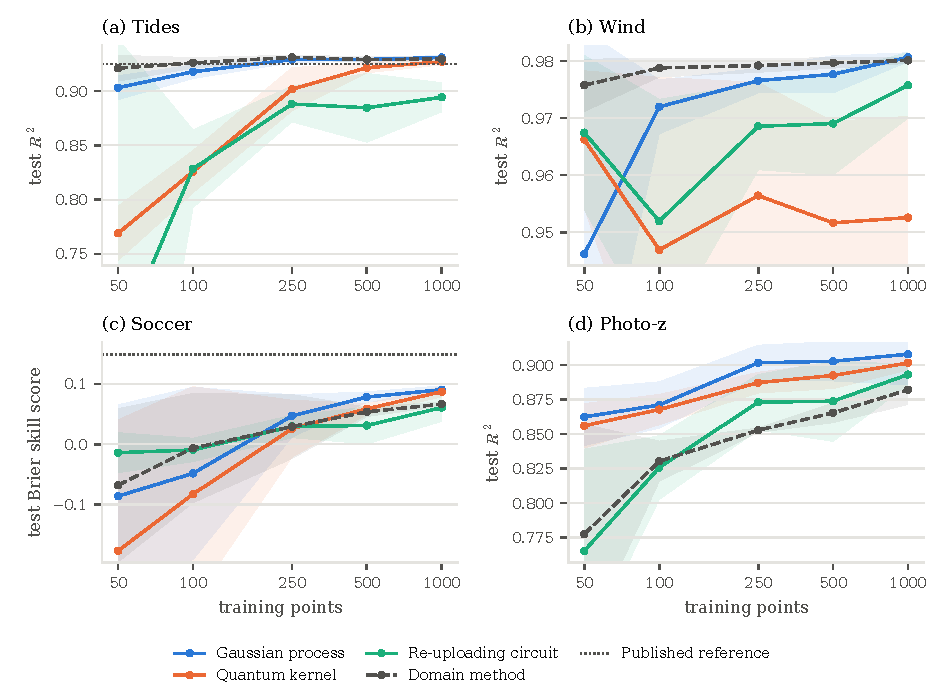
\includegraphics[width=\linewidth]{figures/learning_curves.pdf}
\caption{\label{fig:curves}Test score versus training-set size for the best classical model
(Gaussian process), the two quantum models and the domain method. Lines show the mean and
shaded bands one standard deviation over five seeds; dotted lines mark published references.
Points below the plotted range are clipped.}
\end{figure}

\subsection{Overall comparison}

\Cref{tab:n1000} and \cref{fig:curves} summarize the main result: no quantum model is the
best-performing model on any dataset or at any training-set size (see also \cref{tab:n100}).
The quantum kernel comes closest. With 1000 training points it reaches $R^2=\tidesQK$ on
tides, against \tidesBestCl{} for the best classical model and \tidesDom{} for harmonic
analysis, and exceeds NOAA's official prediction ($\tidesNOAA$) for the test year. On the
redshift control it reaches \photozQK{}, against \photozBestCl{}. On wind, where the target is
dominated by the power curve, all flexible models perform similarly and the domain method
reaches \windDom{}. The re-uploading circuit reaches \windVQC{} there but falls behind on tides
(\tidesVQC{}). On soccer the best trained models attain a Brier skill score of about 0.09,
well below StatsBomb's xG (\soccerSB{}), which draws on information absent from our features,
such as the positions of defenders and the goalkeeper. At small training-set sizes the Gaussian
process and the domain methods are the most reliable; the quantum kernel needs a few hundred
points to approach them, and the variational circuit and the multilayer perceptron vary most
across seeds.

\subsection{Choice of feature map}

The tuner was free to choose between the angle and IQP feature maps. It selected the angle
map in \qkAngleTides{} of \qkRunsTides{} tides runs and \qkAngleWind{} of \qkRunsWind{} wind
runs, but in only \qkAnglePhotoz{} of \qkRunsPhotoz{} redshift runs. The explanation is
structural. The IQP map rotates qubit pairs by products $x_jx_k$; for angles spanning
$[-\pi,\pi)$ these products are not $2\pi$-periodic in either argument, so the resulting
kernel does not respect the periodicity of the inputs. Without tuning, the IQP kernel
achieved $R^2\le 0$ on tides. Rescaling the inputs cannot repair this without destroying the
periodicity of each angle, so the commonly used IQP map is a poor default for periodic data.

\subsection{Spectral analysis of the tidal problem}

\begin{table}[t]
\centering\small
\caption{\label{tab:ceil}Spectrum ceilings for tides: test $R^2$ of the least-squares fit on
each frequency set, using all training hours. $\Omega_1^{\mathrm{add}}\subset\Omega_1$
contains only frequencies with a single nonzero component.}
\begin{tabular}{@{}llrc@{}}
\toprule
Set & Model with this spectrum & Frequencies & Ceiling $R^2$ \\
\midrule
$\Omega_1^{\mathrm{add}}$ & single-feature terms only & 5 & 0.899 \\
$\Omega_1$ & one-layer circuit, angle kernel & 121 & 0.932 \\
$\Omega_2$ & two-layer circuit & 1,562 & 0.941 \\
\bottomrule
\end{tabular}

\end{table}

\begin{figure}[t]
\centering
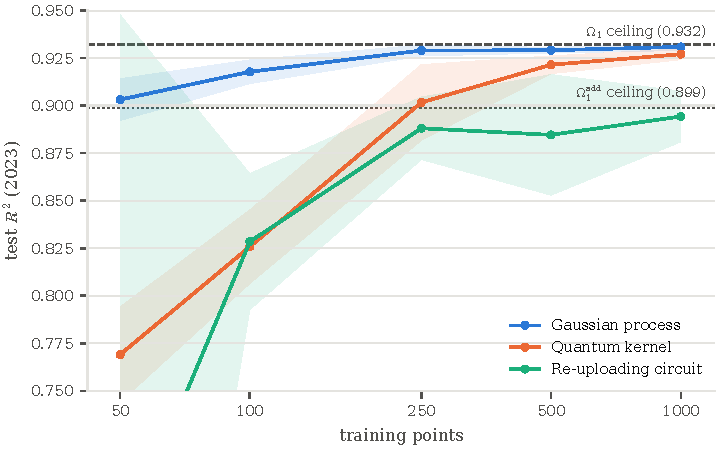
\includegraphics[width=0.72\linewidth]{figures/tides_ceiling.pdf}
\caption{\label{fig:ceiling}Tides: models compared with the spectrum ceilings of
\cref{tab:ceil}. The one-layer ceiling is reached by the classical and kernel models but not
by the variational circuit.}
\end{figure}

\begin{table}[t]
\centering\small
\caption{\label{tab:probe}Re-uploading circuits trained on tides ($n=1000$, seed 0). The short
budget is 100 epochs with patience 15; the long budget is 600 epochs with patience 60. The
\emph{teacher} target is the noise-free least-squares fit on $\Omega_1$, against which its
$R^2$ is measured. $P_2$ is the share of the model's variance at frequencies with
$\max_j|\omega_j|=2$.}
\begin{tabular}{@{}rllrccr@{}}
\toprule
$L$ & Budget & Target & Epochs & Train $R^2$ & Test $R^2$ & $P_2$ (\%) \\
\midrule
1 & short & data & 23 & 0.891 & 0.833 & 0 \\
1 & long & data & 161 & 0.941 & 0.905 & 0 \\
2 & long & data & 86 & 0.701 & 0.563 & 32 \\
3 & long & data & 117 & 0.675 & 0.544 & 29 \\
1 & long & teacher & 375 & 0.971 & 0.967 & 0 \\
2 & long & teacher & 164 & 0.705 & 0.592 & 34 \\
\bottomrule
\end{tabular}

\end{table}

The tuned circuit used a single layer in \vqcOneLayerTides{} of \vqcRunsTides{} tides runs and
remained below ridge regression, which raises the question of whether a single layer simply
lacks the frequencies the tides require. The ceilings in \cref{tab:ceil} rule this out. The
one-layer spectrum $\Omega_1$ supports a test $R^2$ of \ceilOne{}, equal to the best model in
the benchmark, and enlarging it to $\Omega_2$ adds less than 0.01. What matters is not higher
harmonics but interactions: restricting $\Omega_1$ to single-feature frequencies lowers the
ceiling to \ceilAdd{}, because combinations of the five input phases reproduce constituents
that are not themselves inputs. The angle kernel of Eq.~\eqref{eq:anglekernel}, whose spectrum
is exactly $\Omega_1$, is therefore well matched to the problem, consistent with its
performance (\cref{fig:ceiling}).

\Cref{tab:probe} locates the shortfall of the variational model. With a short training
budget, early stopping ends training after 23 epochs and the circuit reaches a test $R^2$ of
0.833. With a longer budget, the same circuit reaches 0.905. Even when trained on a
noise-free target that lies inside its spectrum, the circuit recovers only about 97\% of the
target's variance: $\Omega_1$ comprises 243 real Fourier coefficients, whereas the one-layer
ansatz has 32 parameters and cannot set them independently. Deeper circuits perform worse
rather than better. With $L=2$ or $3$, roughly 30\% of the model's variance lies at frequencies
with $\max_j|\omega_j|=2$, which the data do not require, and training $R^2$ falls to about
0.7. In every case the model spectrum vanishes above $L$ to numerical precision, as
Eq.~\eqref{eq:fourier} predicts.

The full benchmark confirms the role of training. A first run of the benchmark used the short
budget; repeating every variational run with the longer budget described in
\cref{sec:models} raised the circuit's mean tides score at $n=1000$ from \tidesVQCvOne{} to
\tidesVQC{} and halved its spread across seeds (from \tidesVQCvOneSd{} to \tidesVQCSd{}),
with similar gains at small training-set sizes on wind and redshift and little change on
soccer. The circuit nevertheless remains below both the ceiling and ridge regression. Its final
fits on tides ran for a median of \tidesVQCEpochs{} of the \vqcEpochs{} permitted epochs, so it
was most likely still improving when training stopped.

\subsection{Computational cost}

Training the re-uploading circuits accounted for \vqcHours{} of the \allHours{} CPU-hours
used by the entire benchmark. The quantum kernels required only minutes, because states were
simulated once per input.

% ==========================================================================================
\section{Discussion}

Our results support the periodic-input hypothesis only in a weak form. The angle-map quantum
kernel is a sound model for angular data: its spectrum matches what the tidal problem
requires, and it is competitive with the best classical models. However, that kernel is the
simple, classically computable product of Eq.~\eqref{eq:anglekernel}, so its success is not
evidence of a quantum advantage. The variational circuit has an equally appropriate spectrum
but is harder to train, cannot reach every coefficient within that spectrum, and is harmed by
the additional frequencies that deeper circuits introduce. The spectral analysis of
\cref{sec:spectral} makes these distinctions measurable: comparing a ceiling with a model's
score separates limits of the spectrum from limits of training or of the ansatz.

Several limitations qualify these conclusions. All circuits were simulated without hardware or
shot noise. Simulation cost restricted training sets to at most 1000 points and tuning to ten
trials per run. The tidal analysis uses a single station and a single test year. The soccer
data combine four tournaments, and the spectroscopic redshift sample is biased toward bright
galaxies, as is common for photometric-redshift training sets. The variational circuits
were limited to \vqcEpochs{} training epochs, which most tides fits nearly exhausted. Finally,
the probes in \cref{tab:probe} use a single seed, so their exact values are indicative only.

\section{Conclusion}

On four real regression problems, under an equal tuning budget, we find no advantage for
quantum models. We do find that the Fourier picture of quantum models is predictive in
practice: it explains which feature map suits which data, and it separates expressivity from
trainability as the reason a variational circuit falls short. Natural next steps are to
assess robustness to shot noise, to extend the tidal analysis to other stations, and to use
spectrum ceilings to guide the design of circuits and feature maps before training.

\section*{Acknowledgments}
We thank NOAA CO-OPS, Cubico Sustainable Investments, StatsBomb and the Sloan Digital Sky
Survey for making their data openly available. Funding for the Sloan Digital Sky Survey is
acknowledged as described at \url{https://www.sdss.org/collaboration/citing-sdss/}.

\section*{Data and code availability}
All data are public (\cref{tab:data}). The code, configuration files and scripts that produce
every table, figure and number in this paper are available at
\textit{[repository link]}.

\bibliographystyle{unsrtnat}
\bibliography{refs}

\clearpage
\appendix

\section{Hyperparameter search spaces}
\label{app:spaces}

\begin{table}[H]
\centering\small
\caption{\label{tab:spaces}Hyperparameters tuned for each model, with ten trials per run.
UTide, the logistic xG model and the published references have no tuned hyperparameters.}
\begin{tabular}{@{}lll@{}}
\toprule
Model & Hyperparameter & Range \\
\midrule
Ridge / logistic & \texttt{alpha} & $[10^{-4}, 100]$, log \\
Random Fourier features & \texttt{n\_components} & $[50, 500]$, integer \\
 & \texttt{gamma} & $[0.01, 10]$, log \\
 & \texttt{alpha} & $[10^{-4}, 100]$, log \\
Multilayer perceptron & \texttt{hidden} & $[8, 128]$, integer \\
 & \texttt{layers} & $[1, 3]$, integer \\
 & \texttt{alpha} & $[10^{-6}, 0.1]$, log \\
 & \texttt{lr} & $[10^{-4}, 0.01]$, log \\
Gradient boosting & \texttt{max\_depth} & $[2, 8]$, integer \\
 & \texttt{lr} & $[0.01, 0.3]$, log \\
 & \texttt{max\_iter} & $[50, 500]$, integer \\
Gaussian process & \multicolumn{2}{l}{none (marginal likelihood)} \\
Re-uploading circuit & \texttt{n\_layers} & $[1, 4]$, integer \\
 & \texttt{lr} & $[10^{-3}, 0.1]$, log \\
Quantum kernel & \texttt{feature\_map} & \{angle, iqp\} \\
 & \texttt{reps} & $[1, 3]$, integer \\
 & \texttt{bandwidth} & $[0.05, 2]$, log \\
 & \texttt{alpha} & $[10^{-6}, 1]$, log \\
Wind: power curve & \texttt{bin\_width} & $[0.25, 1.5]$, linear \\
Photo-z: knn & \texttt{k} & $[3, 50]$, integer \\
\bottomrule
\end{tabular}

\end{table}

\section{Results with 100 training points}

\begin{table}[H]
\centering\small\setlength{\tabcolsep}{4.5pt}
\caption{Test scores with $n=100$ training points: mean $\pm$ standard deviation over five seeds (higher is better). Bold marks the best model trained on the same points. $R^2$ for regression; BSS is the Brier skill score relative to the base rate, for the probability task.}\label{tab:n100}
\begin{tabular}{@{}llcccc@{}}
\toprule
 & Model & Tides ($R^2$) & Wind ($R^2$) & Soccer (BSS) & Photo-$z$ ($R^2$) \\
\midrule
Classical & Ridge / logistic & $0.891\pm0.012$ & $0.889\pm0.018$ & \best{$0.010\pm0.076$} & $0.772\pm0.055$ \\
 & Random Fourier features & $0.894\pm0.024$ & $0.959\pm0.027$ & $-0.021\pm0.114$ & $0.803\pm0.098$ \\
 & Multilayer perceptron & $0.880\pm0.011$ & $0.928\pm0.023$ & $-0.564\pm0.505$ & $-0.268\pm1.376$ \\
 & Gradient boosting & $0.838\pm0.020$ & $0.825\pm0.050$ & $-0.015\pm0.045$ & $0.835\pm0.008$ \\
 & Gaussian process & $0.918\pm0.006$ & $0.972\pm0.005$ & $-0.048\pm0.143$ & \best{$0.871\pm0.017$} \\
\midrule
Quantum & Re-uploading circuit & $0.828\pm0.036$ & $0.952\pm0.021$ & $-0.009\pm0.019$ & $0.826\pm0.023$ \\
 & Quantum kernel & $0.826\pm0.019$ & $0.947\pm0.030$ & $-0.083\pm0.178$ & $0.868\pm0.011$ \\
\midrule
Domain & Domain method$^{a}$ & \best{$0.926\pm0.005$} & \best{$0.979\pm0.002$} & $-0.006\pm0.090$ & $0.830\pm0.015$ \\
 & Published reference$^{b}$ & $0.925$ & --- & $0.149$ & --- \\
\bottomrule
\end{tabular}
\par\smallskip\begin{minipage}{\linewidth}\footnotesize $^{a}$UTide harmonic analysis (tides), binned power curve (wind), distance--angle logistic regression (soccer) and $k$-nearest neighbours (photo-$z$), fitted on the same training points as every other model. $^{b}$NOAA's official tide prediction and StatsBomb's expected-goals model; both are fitted on far more data and mark a practical ceiling rather than a competitor.\end{minipage}
\end{table}


\end{document}
